\documentclass[main.tex]{subfiles}
\begin{document}

世界是多姿多彩的,而姿需图,彩即色.先说色.
“ 五颜六色”是一个汉语成语,形容色彩复杂或花样繁多,但数字5和6并无确切的含义.“ 
五彩缤纷、万紫千红”里面的5、1,000和10,000也如此.但色彩需要数学来准确地描述.古人以最突出的七种颜色的合称“七彩”,则是确有所指,来自彩虹.
采用传统中国文化说法,毛泽东把它们写进了诗:“ 赤橙黄绿青蓝紫\footnote{赤橙黄绿青蓝紫: red, orange, yellow, green, cyan,blue, purple.},谁持彩练当空舞?”\footnote{《菩萨蛮·大柏地》}赤就是红,而青色就是偏蓝的绿色.在不同的场合见到的彩虹色彩会不同,而且色谱是连续变化的.色谱段的一种取舍可以使主要颜色符合这个顺序.
现在更被采纳的彩虹主要颜色顺序是红橙黄绿蓝靛紫,牛顿是把这个当作日光光谱主要颜色的顺序.牛顿先把日光光谱的主要颜色分为五种:红黄绿蓝紫,
后又相信古希腊人对数字7的推崇,把橙色和靛色加了进去.
日光通过棱镜折出来的光谱与彩虹光谱有所不同,
根据物理学,光谱中的颜色是和光波的波长和频率相对应的.
通过对日光的现代光谱分析,把赤橙黄绿青蓝紫作为日光光谱主要颜色顺序更为恰当.
中国古人和牛顿,正好都相反地小错换了个位.

\begin{figure}
	\centering
	
\includegraphics[width=.98\columnwidth]{eps/rainbow_light_spectrum.eps}
	\caption{HTML/SVG 支持的 141 种颜色}
	\label{fig:1.4.8}
\end{figure}

770~622nm,感觉为红色;622~597nm,橙色;597~577nm,黄色;577~492nm,绿色;492~455nm,蓝靛色;455~390nm,紫色。

SVG\index{SVG, Scalable Vector Graphics} 1.1定义了147 种颜色的英文名\footnote{https://www.w3.org/TR/SVG11/types.html}.
所有浏览器都支持 HTML/CSS 使用其中 141 种颜色的英文名.
用 Python 编程 SVG 生成的这些颜色如 图\ref{fig:1.4.2}.
但对比实际生成的颜色发现,个别用英文名生成的颜色有偏差,如 FireBrick (耐火红砖)和
VioletRed (紫红). 另外也应注意Green (绿色 \#{}008000)和Lime (鲜绿色 \#{}00FF00)的确切 RGB 定义. RGB 是我们接着要讨论的.

\begin{figure}
	\centering
	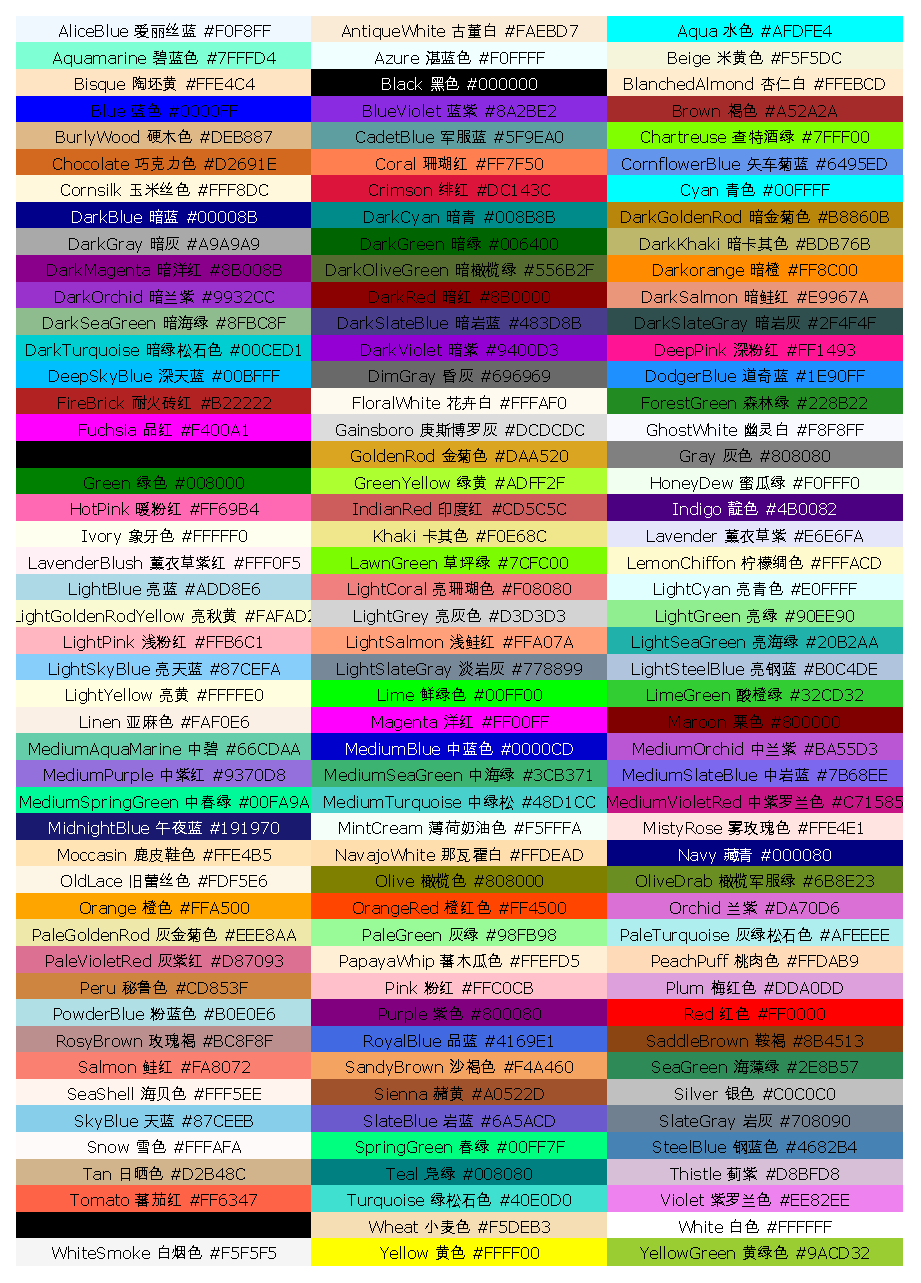
\includegraphics[width=.98\columnwidth]{eps/html_colors.eps}
	\caption{HTML/SVG 支持的 141 种颜色}
	\label{fig:1.4.2}
\end{figure}

最常用的则是 HTML 的 16 种基本颜色, 如 图\ref{fig:1.4.3}.

\begin{figure}
	\centering
	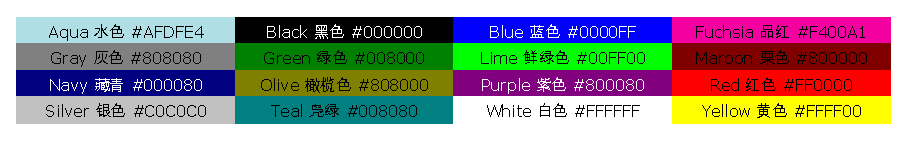
\includegraphics[width=.98\columnwidth]{eps/html_16colors.eps}
	\caption{HTML的 16 种基本颜色}
	\label{fig:1.4.3}
\end{figure}

cyan = 1.0 - red

magenta = 1.0 - green

yellow = 1.0 - blue

indigo \#4B0082 75, 0, 130

\begin{figure}
	\centering
	
\includegraphics[width=0.5\columnwidth]{svg/simple_example.eps}
	\caption{简单例子}
	\label{fig:I.1.}
\end{figure}



爱丽丝蓝%#F0F8FF
古董白%#FAEBD7
水色%#00FFFF
海蓝宝石% #7FFFD4
天蓝色%#F0FFFF
米色% #F5F5DC
浓汤%#FFE4C4

\newpage
\end{document} 
